%!TEX root = Slic3r-Manual.tex
\section{Mode Simple} % (fold)
\label{sec:simple_mode}
\index{simple mode}
\index{mode simple}

Slic3r a deux modes de fonctionnement, Simple et Expert. Ceux-ci peuvent \^etre choisis \`a partir de la fen\^etre \texttt{Prefer\'ences} (qui se trouve dans le menu  \texttt{File} (fichier) ).

\begin{figure}[ht]
\centering
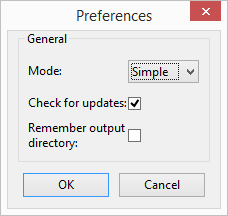
\includegraphics[width=0.3\textwidth]{simple_mode/preferences_general.png}
\caption{Pref\'erences.}
\label{fig:preferences_general}
\end{figure}

Le mode simple offre une gamme r\'eduite de param\`etres, suffisament pour que le d\'ebutant puisse commencer. Le mode expert donne plus de contr\^ole sur la mani\`ere dont Slic3r produit le G-code, celui-ci sera examin\'e plus tard.

\section{Param\`etres d'Impression}
\index{Print Settings}
\index{Param\`etres d'Impression}

L'onglet \texttt{Print Settings} (param\`etres d'impression) 
offre la possibilit\'e de modifier les param\`etres li\'es \`a l'impression r\'eelle. Alors que les autres onglets sont modifi\'ees moins souvent, les param\`etres de cet onglet seront modifi\'es r\'eguli\`erement, \'eventuellement pour chaque mod\`ele imprim\'e.

\begin{figure}[ht]
\centering
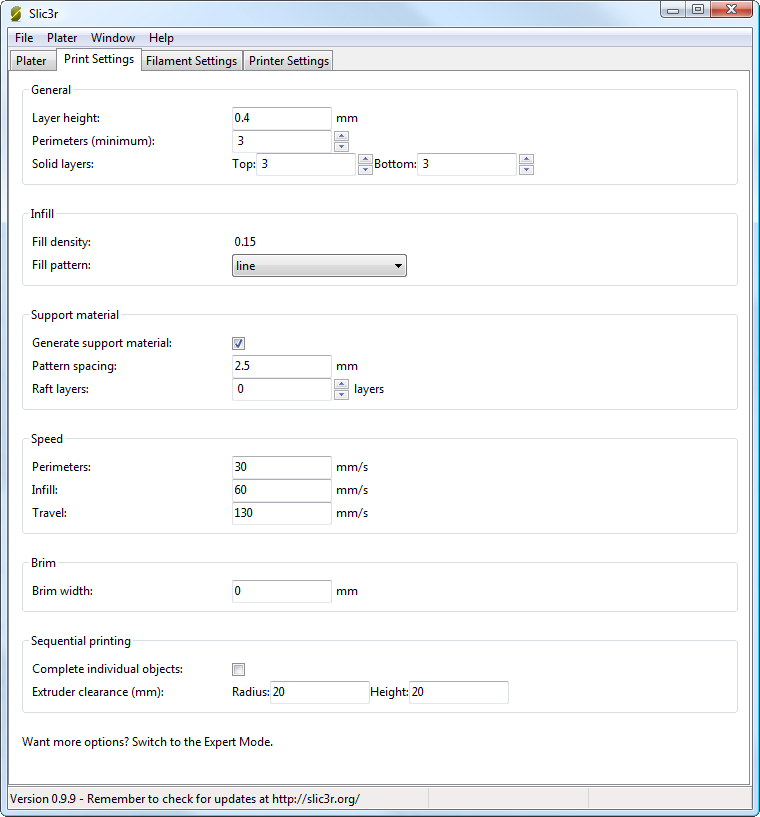
\includegraphics[width=\textwidth]{simple_mode/simple_mode_print_settings.png}
\caption{Mode Simple: Param\`etres d'impression.}
\label{fig:simple_mode_print_settings}
\end{figure}

\paragraph{G\'en\'eral.} % (fold)
\label{par:simple_general}
\index{Print Settings!Layer height}
\index{Param\`etres d'Impression!Epaisseur de couche}

\texttt{Layer height} (\'epaisseur de couche) d\'efinit le d\'eplacement sur l'axe vertical avant l'extrusion d'une nouvelle couche.  Il y a plusieurs facteurs qui influentsur la hauteur que la couche doit avoir:
\begin{itemize}
	\item \textbf{R\'esolution D\'esir\'ee}  - Une faible hauteur de couche devrait conduire \`a des impressions avec des nervures ou des bandes moins visibles, comme chaque couche est plus petite. L'esth\'etique joue ici un r\^ole, mais aussi le type de mod\`ele, par exemple, une pi\`ece m\'ecanique peut ne pas avoir besoin d'une telle finition haute r\'esolution, alors qu'une pi\`ece de pr\'esentation peut en avoir besoin.
	\item \textbf{Vitesse d'impression}  - Les couches plus fines produiront des impression lisses, mais chaque impression prendra plus de temps, tout simplement parce que l'extrudeuse doit tracer le motif plusieurs fois. Un des buts plus tard sera de trouver un \'equilibre entre la hauteur de couche, la vitesse de l'imprimante, et la qualit\'e de l'impression qui en r\'esulte.
\end{itemize}
\index{Print Settings!Perimeters}
\index{Param\`etres d'Impression!P\'erim\`etres}
\texttt{Perimeters} (P\'erimetres) d\'efinit le nombre minimum de coquilles verticales (c'est \`a dire les murs) que l'impression aura. \`a moins que le mod\`ele ne n\'ecessite qu'un seul mur, il est g\'en\'eralement recommand\'e d'avoir un minimum de deux p\'erim\`etres car cela donne l'assurance que si une partie du p\'erim\`etre ne s'imprime pas correctement alors le second p\'erim\`etre permettra le de couvrir.

\index{Print Settings!Solid layers}
\index{Param\`etres d'Impression!Couches pleines}
Les couches sup\'erieure et inf\'erieure qui prennent en sandwich le mod\`ele sont remplis de motifs de \texttt{Solid layers} (couches pleines). Pour les couches inf\'erieures (bottom) le facteur important \`a prendre en compte est la façon dont la surface aura l'air s'il y avait une anomalie, lors de l'impression de la premi\`ere couche, c'est pour cette raison, qu'il est recommand\'e d'avoir au moins deux couches inf\'erieures.

Une prise en compte similaire est n\'ecessaire pour les couches sup\'erieures (top). Parce que les couches interm\'ediaires sont susceptibles d'\^etre rempli d'un motif fix\'e \`a moins de 100\% , les couches de rev\^etement devront combler ce motif et cela peut n\'ecessiter plus d'un passage pour le couvrir compl\`etement.

\begin{figure}[H]
\centering
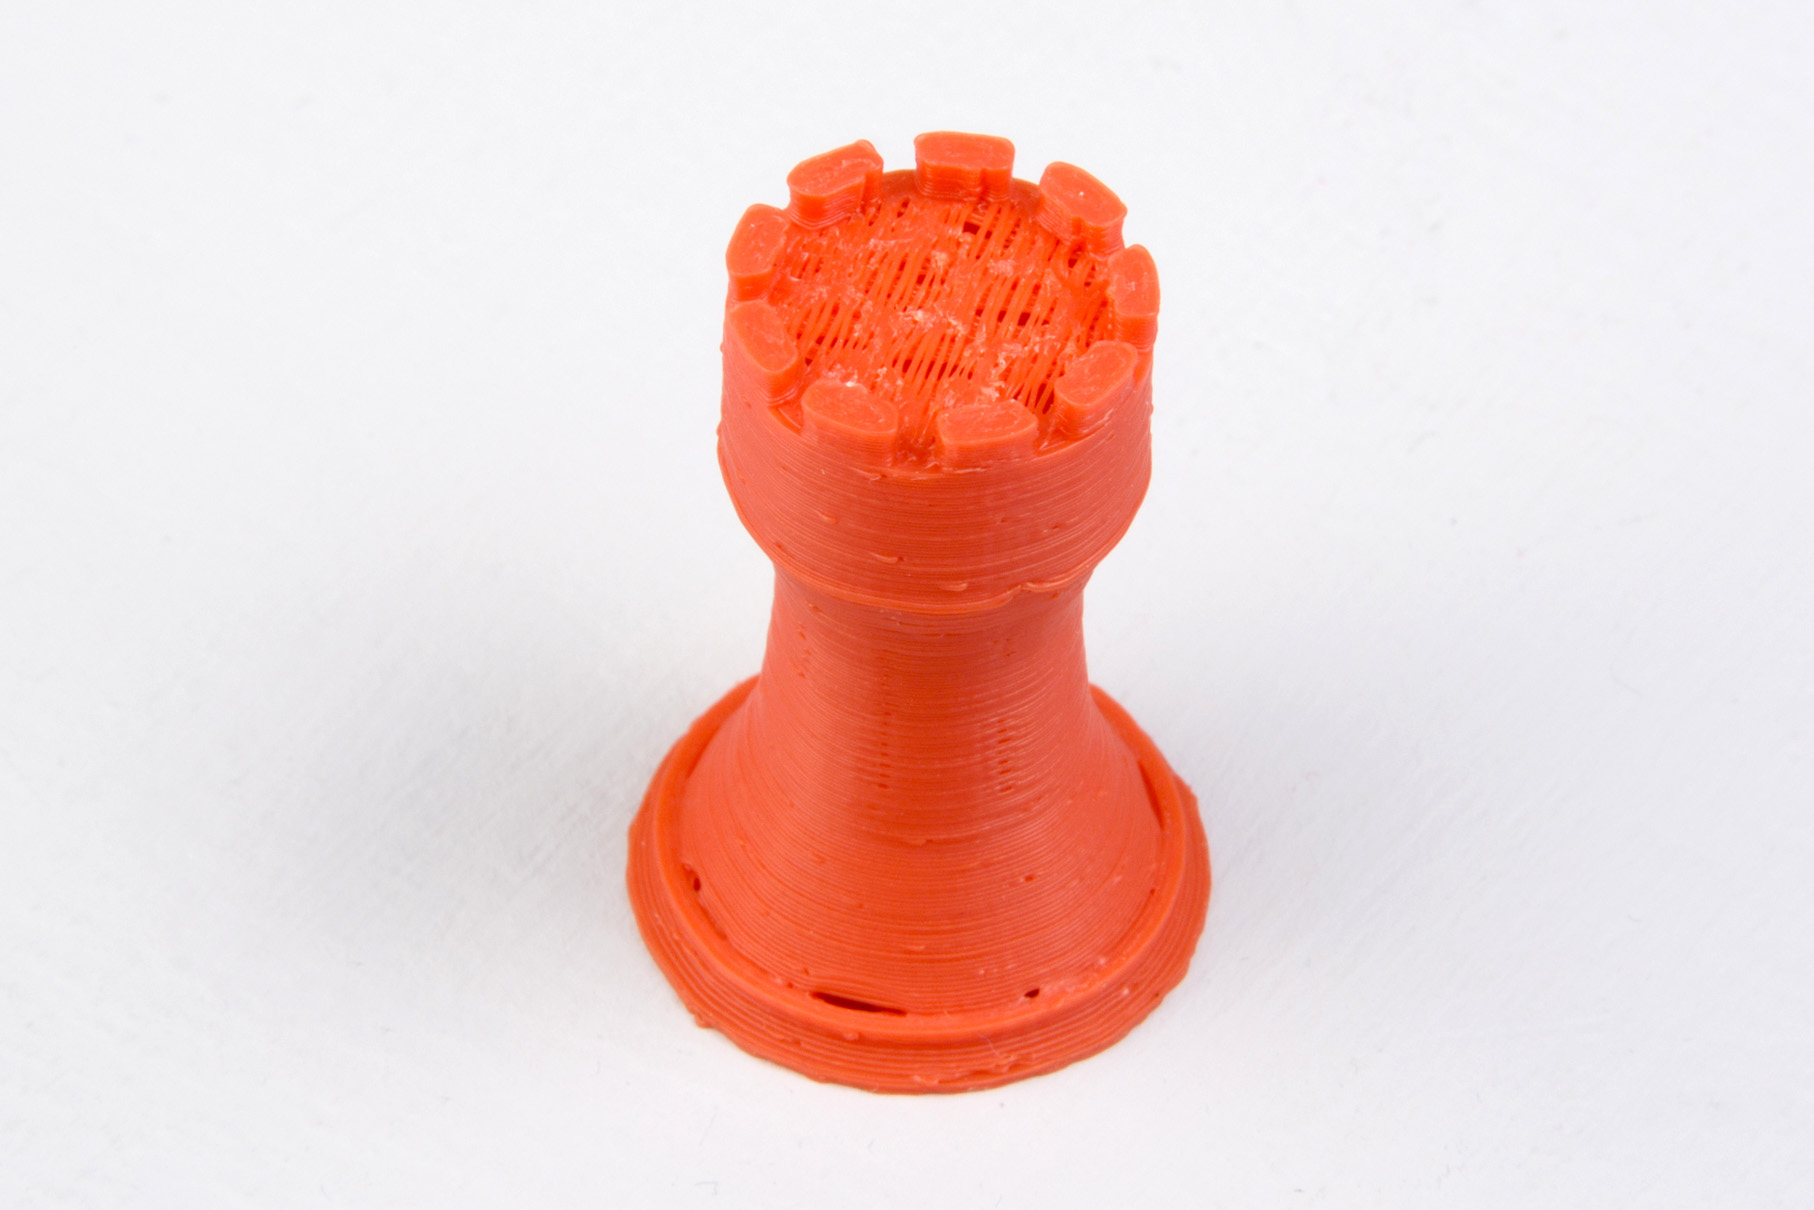
\includegraphics[keepaspectratio=true,width=0.75\textwidth]{simple_mode/bad_top_infill.jpg}
\caption{Un exemple de couches sup\'erieures insuffisantes.}
\label{fig:bad_top_infill}
\end{figure}

Une autre astuce \`a consid\'erer: R\'egler la couche pleine sup\'erieure (top solid layer) \`a z\'ero, et r\'egler le remplissage \'egalement \`a z\'ero, produira un r\'ecipient , id\'eal pour transformer les mod\`eles en vases\footnote{http://slic3r.org/blog/tip-printing-vases} par exemple. Ici la modification des param\`etres peuvent \^etre utilis\'es dans Slic3r pour g\'en\'erer diff\'erents types de impressions, et pas seulement pour contr\^oler la pr\'ecision de surface.

\begin{figure}[H]
\centering
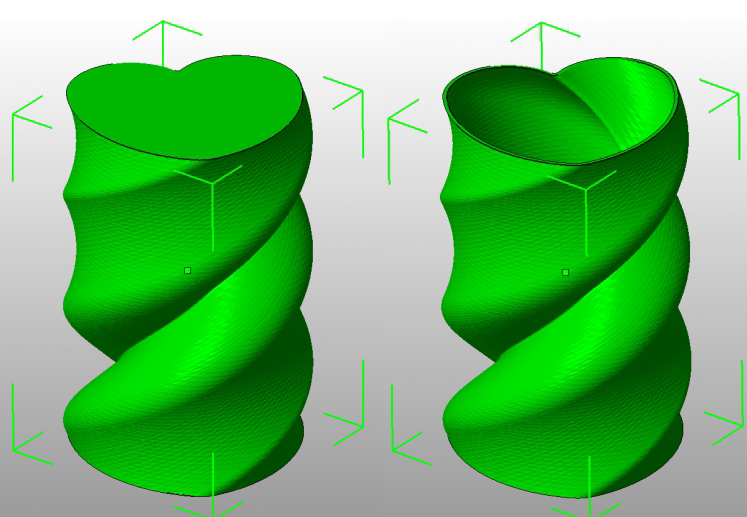
\includegraphics[keepaspectratio=true,width=0.75\textwidth]{simple_mode/solid_layers_vases.png}
\caption{Cr\'eation d'un vase \`a partir d'un mod\`ele solide.}
\label{fig:solid_layers_vases}
\end{figure}

% paragraph general (end)

\paragraph{Remplissage. (Infill)} % (fold)
\label{par:simple_infill}
\index{Print Settings!Infill}
\index{Param\`etres d'Impression!Remplissage}
\index{Print Settings!Infill!Fill density}
\index{Param\`etres d'Impression!Remplissage!Densit\'ee de remplissage}
\texttt{Fill density} (Densit\'e de remplissage) est d\'efinie sur une \'echelle comprise entre 0 et 1, o\`u 1 est de 100\% et 0,4 serait 40\%. Pour la majorit\'e des cas, remplir la pi\`ece \`a 100\% n'a pas d'int\'er\^et, ce serait un gaspillage de mat\'eriel et prendrait beaucoup de temps. Au lieu de cela, la plupart des mod\`eles peuvent \^etre remplis avec moins de mati\`ere, qui sera ensuite pris en sandwich entre les couches remplies \`a 100\% (voir \texttt{Solid layers} au dessus).

Une valeur de densit\'e de 0,4 est suffisant pour donner \`a la quasi-totalit\'e des mod\`eles une bonne r\'esistance m\'ecanique. Une valeur de 0,2 est g\'en\'eralement le minimum requis pour soutenir des plafonds plats.

\index{Print Settings!Infill!Fill pattern}
Slic3r offre plusieurs motifs de remplissage qui seront examin\'es plus en d\'etail dans la section \ref{sec:infill_patterns_and_density} - Motifs et densit\'ee de remplissage.  Choisir un \texttt{Fill pattern} (motif de remplissage) d\'ependra du type de mod\`ele, la r\'esistance souhait\'ee de la structure , la vitesse d'impression, et des go\^uts personnels. Les modes de remplissage plus exotiques sont g\'en\'eralement trop lent et inutilement complexe pour la plupart des cas d'utilisation, et donc la plupart du temps, le motif de remplissage est soit \texttt{rectilinear} (rectiligne), \texttt{line} (ligne), or \texttt{honeycomb} (nid d'abeille).  Honeycomb offre le plus r\'esistance, mais est plus lent que les deux rectilinear ou line.

% paragraph infill (end)

\paragraph{Support. (Support material)} % (fold)
\label{par:simple_support_material}
\index{Print Settings!Support material}
\index{Param\`etres d'Impression!Support}
\index{Print Settings!Support material!Generate support material}
\index{Param\`etres d'Impression!Support!G\'en\'erer le support}
\index{Print Settings!Support material!Pattern spacing}
\index{Param\`etres d'Impression!Support!Espacement du motif}
Imprimer un mod\`ele de bas en haut, avec une imprimante FDM, signifie que les saillies importantes seront imprim\'ees dans le vide, pruduisant des affaissement ou un mauvais r\'esultat.  Obter pour un support (\texttt{Generate support material}) ajoutera des structures suppl\'ementaires dans le mod\`ele qui seront construites pour soutenir la partie en surplomb. Le param\`etre \texttt{Pattern spacing} (espacement du motif) d\'etermine la densit\'e du support qui est imprim\'e.

\begin{figure}[H]
\centering
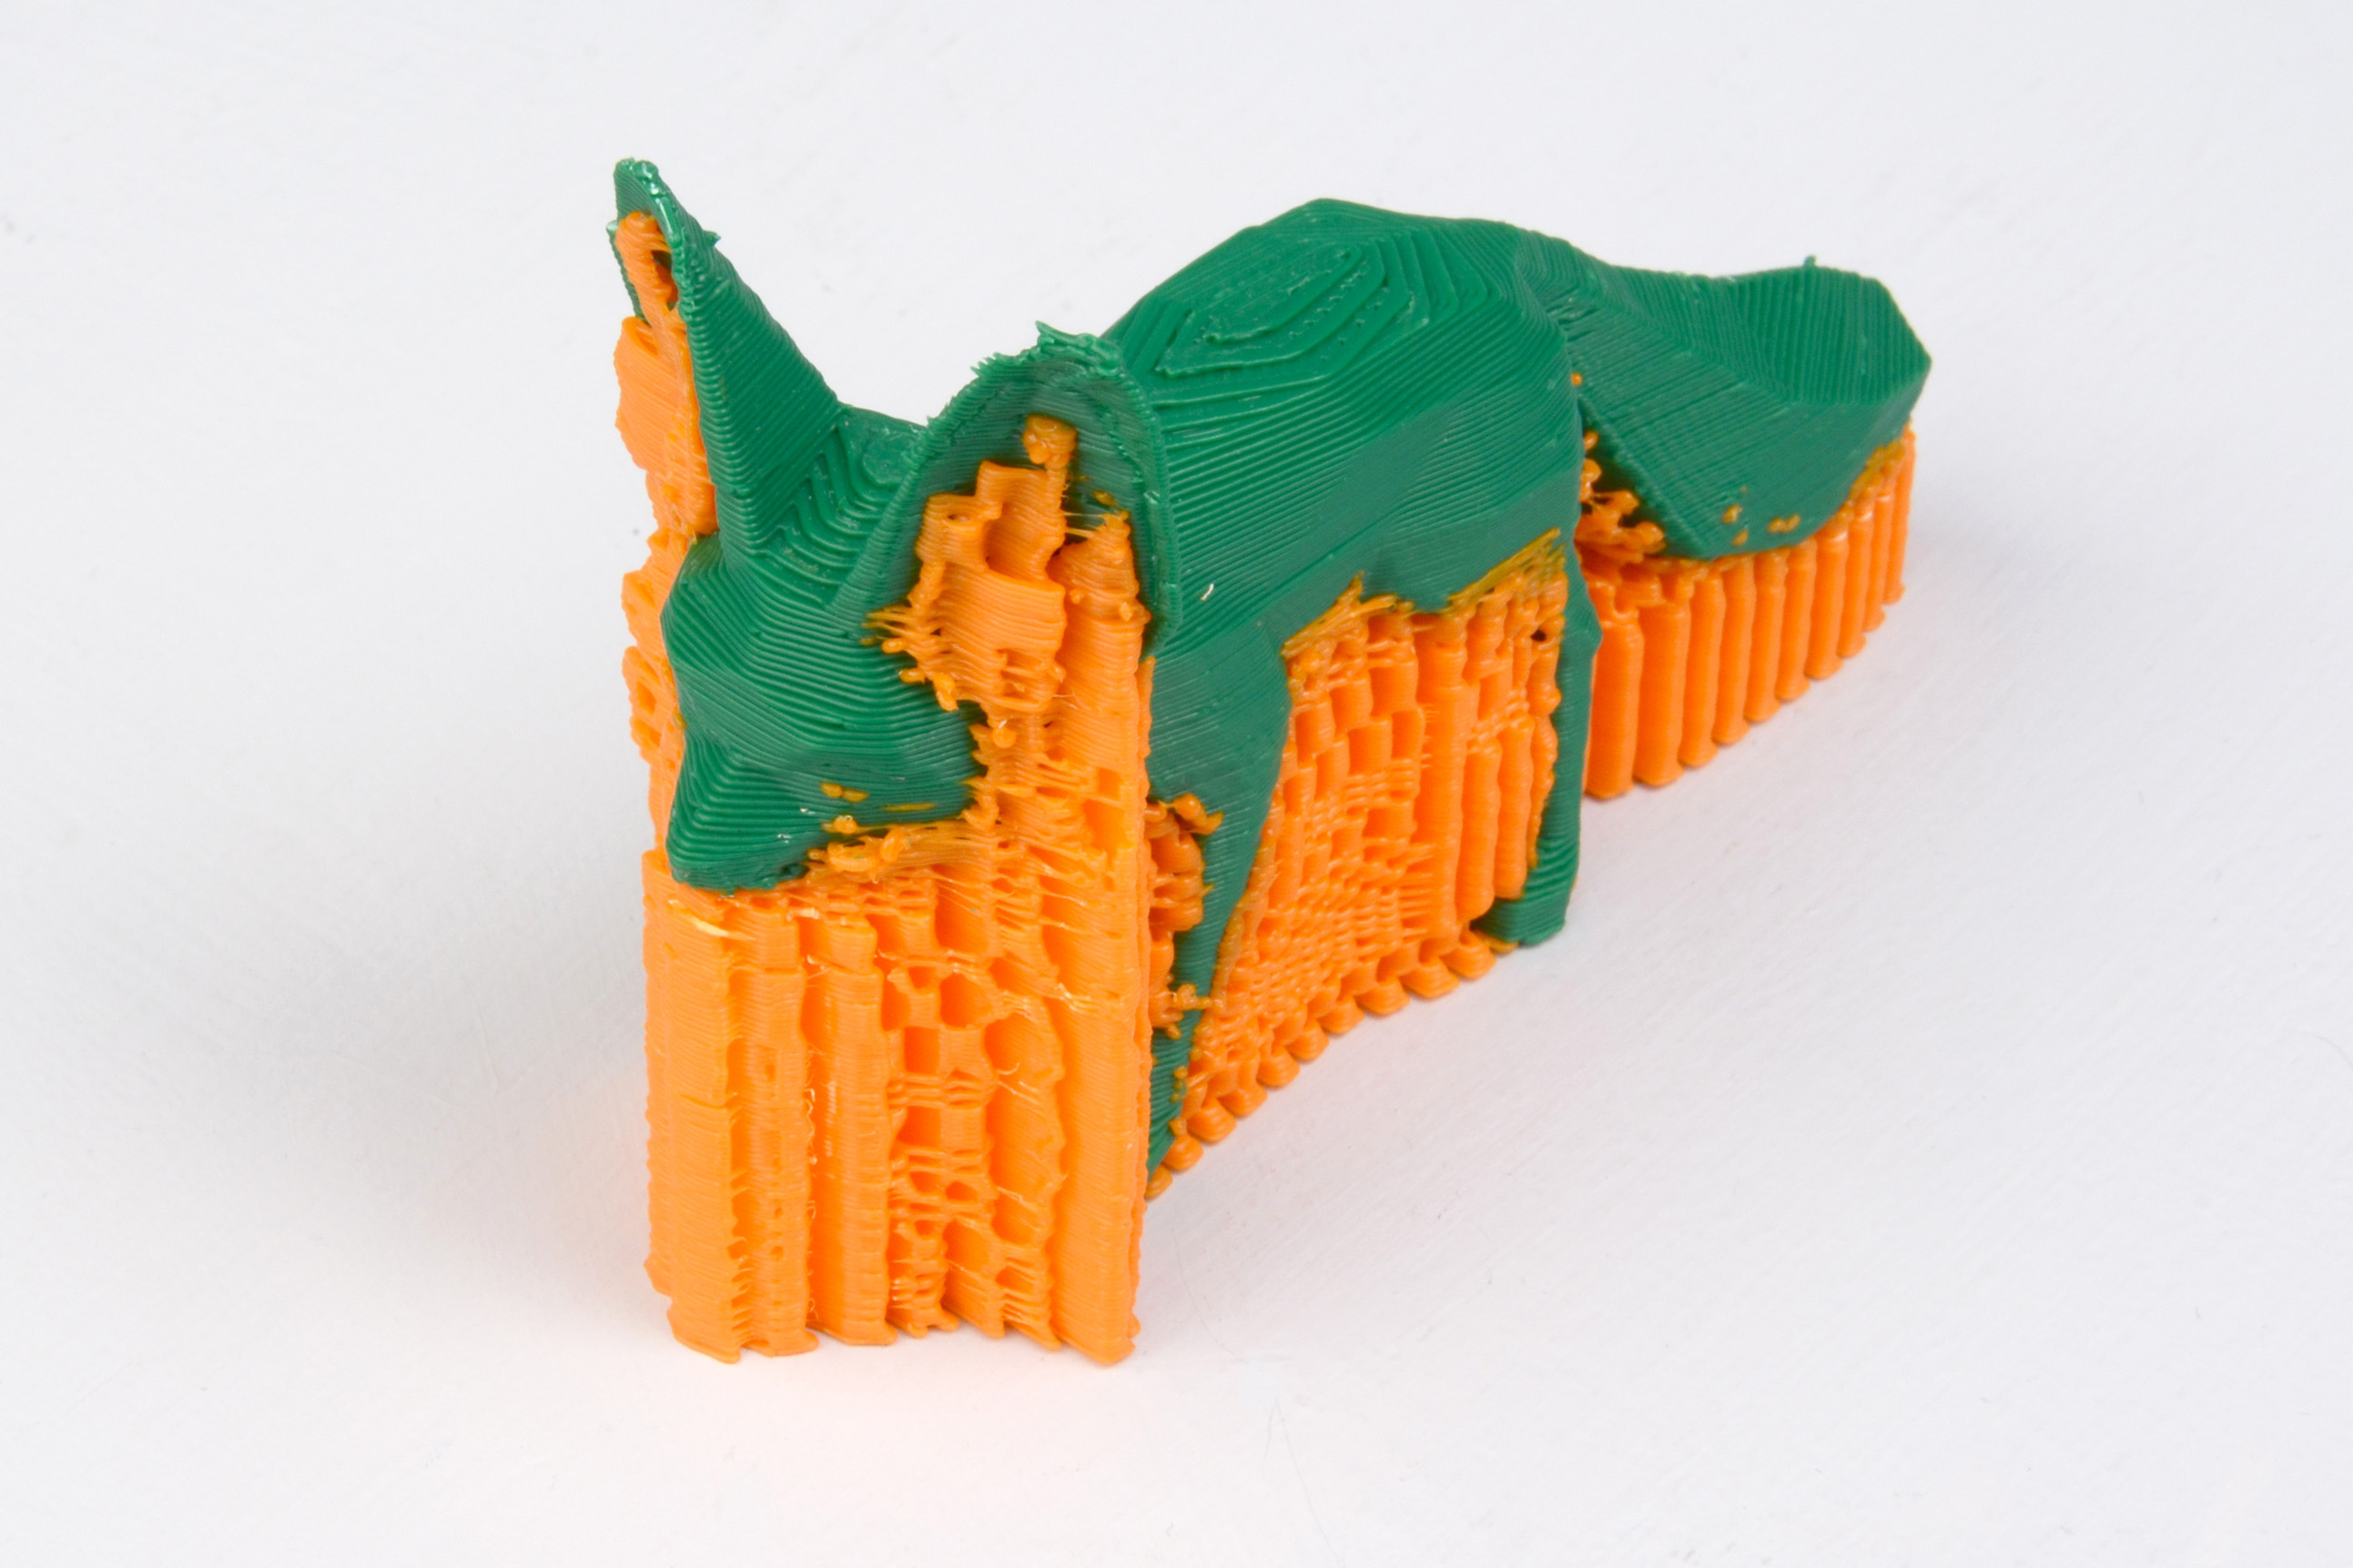
\includegraphics[keepaspectratio=true,width=0.75\textwidth]{simple_mode/support_example.jpg}
\caption{Un exemple d'un objet imprim\'e avec un support.}
\label{fig:support_example}
\end{figure}

Astuce: Il est parfois utile d'envisager de modifier l'orientation du mod\`ele afin de r\'eduire \'eventuellement les surplombs.

\index{Print Settings!Support material!Raft layers}
\index{Param\`etres d'Impression!Support!Radier}
\texttt{Raft layers} (radier) va ajouter des couches suppl\'ementaires sous le mod\`ele et d\'ecoule depuis les d\'ebuts de l'impression 3D. Il peut vous aider \`a imprimer sans lit chauff\'e, ou lorsque le lit n'est pas tr\`es plat, mais il n'est g\'en\'eralement pas n\'ecessaire et n'est pas recommand\'e. Le radier n\'ecessite en outre un post-traitement pour le supprimer.
% paragraph support_material (end)

\paragraph{Vitesse. (Speed)} % (fold)
\label{par:simple_speed}
\index{Print Settings!Speed}
En mode simple, il n'y a que trois r\'eglages de vitesse \`a configurer:
\index{Print Settings!Speed!Perimeters}
\index{Param\`etres d'Impression!P\'erim\`etres}
\index{Print Settings!Speed!Infill}
\index{Param\`etres d'Impression!Vitesse!Remplissage}
\index{Print Settings!Speed!Travel}
\index{Param\`etres d'Impression!Vitesse!D\'eplacement}
\begin{itemize}
	\item \texttt{Perimeters} (Perimeters) - Le contour du mod\`ele peut b\'en\'eficier d'une vitesse d'impression l\'eg\`erement plus lente de sorte que la peau ext\'erieure de l'impression ait moins de d\'efauts.
	\item \texttt{Remplissage} (Infill) - Comme le remplissage est cach\'e il peut \^etre extrud\'e un peu plus vite. Prenez bien soin de ne pas aller trop vite, car plus la vitesse est \'elev\'ee, et plus les extrusions sont minces, et cela peut affecter la façon dont se fait la liaison entre les extrusions.
	\item \texttt{D\'eplacement} (Travel) - Le saut entre la fin d'une extrusion et la suivante doivent g\'en\'eralement \^etre effectu\'ees aussi rapidement que l'imprimante le permet , afin de minimiser les d\'eg\^ats caus\'es par suintement de mat\'eriau depuis la buse.
\end{itemize}
% paragraph speed (end)

\paragraph{Bordure. (Brim)} % (fold)
\label{par:simple_brim}
\index{Print Settings!Brim}
\index{Param\`etres d'Impression!Bordure}
\index{Print Settings!Brim!Brim width}
\index{Param\`etres d'Impression!Bordure!Largeur de bordure}
\texttt{Brim width} (largeur de bordure) est utilis\'e pour ajouter plus de p\'erim\`etres \`a la premi\`ere couche, en tant base suppl\'ementaire, afin de fournir une plus grande surface pour que l'impression colle au lit , afin de r\'eduire les d\'eformation (voir §\ref{sec:the_important_first_layer}). Le bord est ensuite d\'ecoup\'ee une fois que l'impression est termin\'ee et retir\'ee du lit.

\begin{figure}[H]
\centering
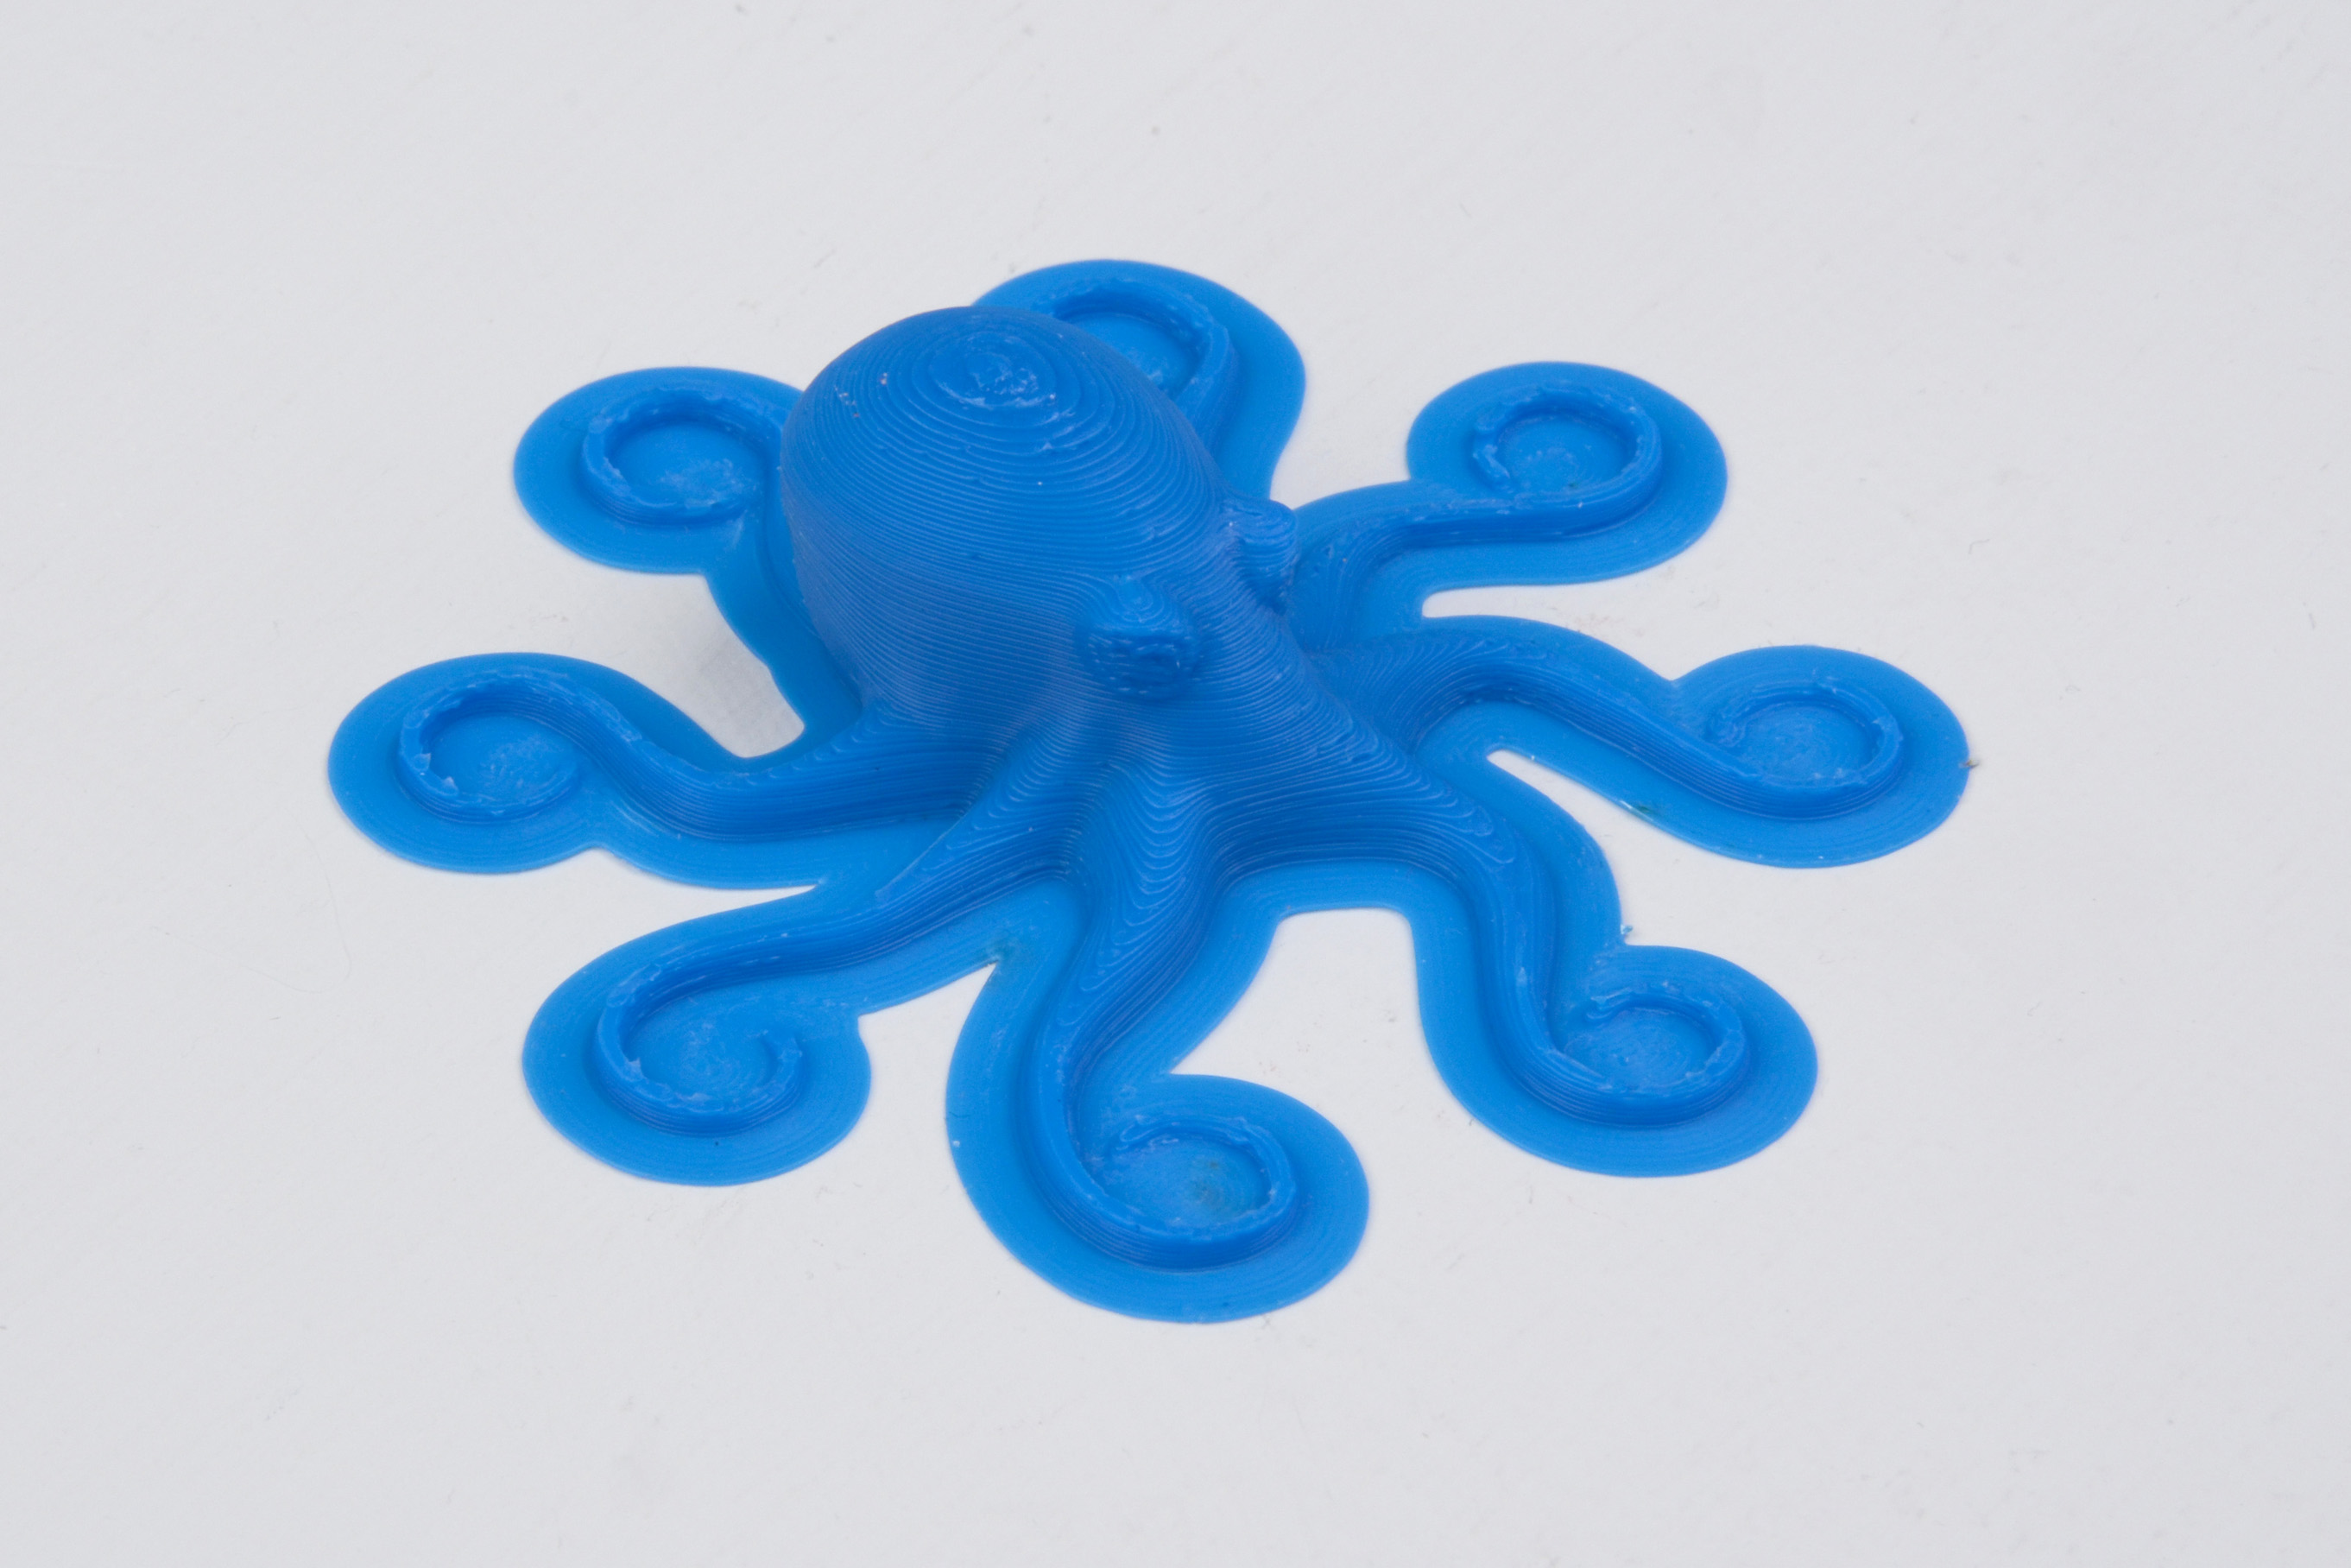
\includegraphics[keepaspectratio=true,width=0.75\textwidth]{simple_mode/brim.jpg}
\caption{Un exemple de bordure.}
\label{fig:an_example_of_brim}
\end{figure}

% paragraph brim (end)

\paragraph{Impression Sequentielle.} % (fold)
\label{par:sequential_printing}
Cette fonction permet de composer un plateau d'objets, en imprimant compl\'etement chaque pi\`ece individuellement, avant de revenir \`a Z = 0 et de continuer par le suivant. Voir la section sur l'impression s\'equentielle dans le chapitre des sujets avanc\'es.


\section{Param\`etres du Filament}
\index{Filament Settings}
\index{Param\`etres du Filament}
L'onglet \texttt{Filament Settings} (Param\`etres du Filament) sera normalement utilis\'e peu fr\'equemment, par exemple lors de la r\'eception d'un nouveau rouleau de filament.

\begin{figure}[H]
\centering
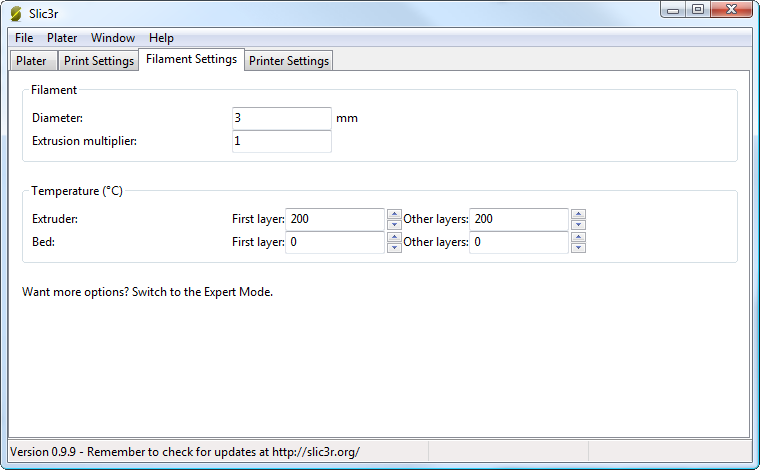
\includegraphics[width=\textwidth]{simple_mode/simple_mode_filament_settings.png}
\caption{Mode Simple: Param\`etres du Filament.}
\label{fig:simple_mode_filament_settings}
\end{figure}

\paragraph{Filament.} % (fold)
\label{par:filament}
\index{Filament Settings!Filament}
\index{Param\`etres du Filament!Filament}
\index{Filament Settings!Filament!Diameter}
\index{Param\`etres du Filament!Filament!Diam\`etre}
Le param\`etre \texttt{Diameter} (Diam\`etre) aura d\'ej\`a \'et\'e rempli \`a partir de la valeur donn\'ee au cours de l'assistant (voir p.\pageref{sub:4_filament_diameter}), mais peut \^etre modifi\'ee ici.

\index{Filament Settings!Filament!Extrusion multiplier}
\index{Param\`etres du Filament!Filament!Multiplicateur d'Extrusion}
La param\`etre \texttt{Extrusion multiplier} (Multiplicateur d'Extrusion) permet le r\'eglage fin de la vitesse d'\'ecoulement d'extrusion, et est est donn\'ee en tant que facteur, par exemple, 1 signifie 100 \%, 1,5 signifierait 150 \%. Alors que la valeur devrait id\'ealement \^etre d\'efinie dans le firmware, il peut \^etre utile de tester l\'eg\`eres modifications de la vitesse en modifiant cette valeur. Elle modifie la quantit\'e de plastique en proportion et doit \^etre chang\'e par de tr\`es petites \'etapes (par exemple + / - 0,05) car les effets sont tr\`es visibles.
% paragraph filament (end)

\paragraph{Temp\'erature.} % (fold)
\label{par:temperature}
\index{Filament Settings!Temperature!Extruder}
\index{Param\`etres du Filament!Temp\'erature!Extrudeuse}
\index{Filament Settings!Temperature!Bed}
\index{Param\`etres du Filament!Temp\'erature!Lit}
Ces valeurs sont \'egalement d\'efinies \`a partir de l'assistant, mais ici la possibilit\'e existe de r\'egler la temp\'erature de la premi\`ere couche (voir p.\pageref{sec:the_important_first_layer}).
% paragraph temperature (end)


\section{Param\`etres de l'Imprimante}
\index{Printer Settings}
\index{Param\`etres de l'Imprimante}

Les param\`etres de l'imprimante (\texttt{Printer Settings}) ne seront jamais mis \`a jour, \`a moins que Slic3r ne soit utilis\'e pour de nombreuses imprimantes, par exemple, pour une batterie de l'imprimante 3D.

\begin{figure}[H]
\centering
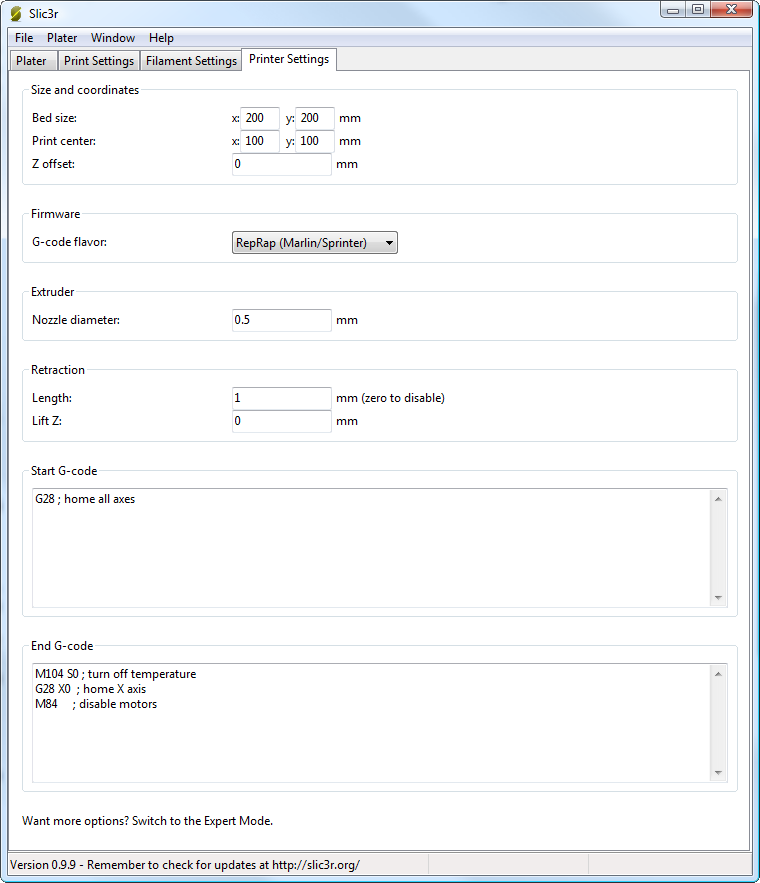
\includegraphics[width=\textwidth]{simple_mode/simple_mode_printer_settings.png}
\caption{Mode Simple: Param\`etres de l'Imprimante.}
\label{fig:simple_mode_printer_settings}
\end{figure}

\paragraph{Size and coordinates. (Taille et coordonn\'ees)} % (fold)
\label{par:size_and_coordinates}
\index{Printer Settings!Size and coordinates}
\index{Param\`etres de l'Imprimante!Taille et coordonn\'ees}
\index{Printer Settings!Size and coordinates!Bed size}
\index{Param\`etres de l'Imprimante!Taille et coordonn\'ees!Taille d lit}
Le param\`etre \texttt{Bed size} (Taille du lit) est repris \`a partir de l'assistant (voir p.\pageref{sub:2_bed_size}) et est utilis\'e seulement pour la pr\'evisualisation du mod\`ele sur la surface de travail.

\index{Printer Settings!Size and coordinates!Print center}
\index{Param\`etres de l'Imprimante!Taille et coordonn\'ees!Centre de l'impression}
Le param\`etre \texttt{Print center} (centre de l'impression) defini le point autour duquel l'impression sera centr\'e.  La taille du lit (\texttt{Bed size}) r\'egl\'ee \`a 200mmx200mm et le centre d'impression (\texttt{Print center}) r\'egl\'e \`a 100mmx100mm would placera l'impression au milieu.  Si l'on souhaite imprimer \`a partir du centre, afin d'eviter des bris sur le rebors du verre, cette option doit \^etre utilis\'ee.

\index{Printer Settings!Size and coordinates!Z offset}
\index{Param\`etres de l'Imprimante!Taille et coordonn\'ees!D\'ecalage Z}
\texttt{Z offset} (d\'ecalage Z) peut \^etre utilis\'e pour compenser une fin de course Z mal calibr\'e. Si la buse s'arr\^ete un peu trop loin du lit, on peu conpenser le d\'ecalage en ajoutant une valeur n\'egative. La bonne solution est de r\'egler la but\'ee.

La position de fin de course Z optimale est l\`a o\`u la buse touche \`a peine la surface du lit quand elle se trouve au point d'origine. Une feuille de papier fait un bon indicateur pour cette tr\`es petite distance. Il n'est pas recommand\'e d'utiliser ce param\`etre pour essayer d'am\'eliorer l'adh\'erence couche, en "\'ecrasant" la couche inf\'erieure sur le lit, regardez plut\^ot les suggestions de la section \ref{sec:the_important_first_layer}.
% paragraph size_and_coordinates (end)

\paragraph{Firmware. (Micrologiciel)} % (fold)
\label{par:firmware}
\index{Printer Settings!Firmware!G-code flavour}
\index{Param\`etres de l'Imprimante!Micrologiciel!Variante du G-code}
Comme renseign\'e par l'assistant (voir p.\pageref{sub:1_firmware_type}), \texttt{G-code flavour} (variante du G-code) d\'efinit le dialecte de G-code g\'en\'er\'e.
% paragraph firmware (end)


\paragraph{Extruder. (Extrudeuse)} % (fold)
\label{par:extruder}
\index{Printer Settings!Extruder!Nozzle diameter}
\index{Param\`etres de l'Imprimante!Extrudeuse!Diam\`etre de la buse}
\texttt{Nozzle diameter} (diam\`etre dela buze) est renseign\'e par l'assistant (voir p.\pageref{sub:3_nozzle_diameter}).
% paragraph extruder (end)

\paragraph{Retraction. (Retractation)} % (fold)
\label{par:retraction}
\index{Printer Settings!Extruder!Retraction!Length}
\index{Param\`etres de l'Imprimante!Extrudeuse!R\'etractation!Longueur}
\`a moins que le mat\'eriau en cours d'extrusion ait une viscosit\'e tr\`es \'elev\'ee, il peut suinter entre extrusions dues \`a la pesanteur. Cela peut \^etre r\'esolu en r\'etractant activement le filament entre les extrusions.  R\'egler le param\`etre \texttt{Length} (longueur) \`a une valeur positive causera le filament \`a \^etre retir\'e de plusieurs millim\`etres avant le d\'eplacement. Le retrait sera alors compens\'ee par la m\^eme quantit\'e apr\`es le d\'em\'enagement de Voyage, avant de commencer le nouveau chemin d'extrusion.

Une valeur comprise entre 1 et 2 mm est habituellement recommand\'e. Extrudeuses sous gaine peuvent avoir besoin de 4 ou 5 mm en raison de l'hyst\'er\'esis introduit par le tube.
\index{Printer Settings!Extruder!Retraction!Lift Z}
\index{Param\`etres de l'Imprimante!Extrudeuse!R\'etractation!\'el\'evation Z}
R\'egler le param\`etre \texttt{Lift Z} (El\'evation Z) \`a une valeur positive rel\`evera l'extrudeuse sur l'axe Z de ce nombre de millim\`etres durant chaque d\'eplacement. Cela peut \^etre utile pour s'assurer que la buse n'accroche pas la couche pr\'ecedente, mais cette valeur n'est g\'en\'eralement pas n\'ecessaire et ralentit la vitesse d'impression. Une valeur de 0,1 mm est g\'en\'eralement suffisante.
% paragraph retraction (end)

\paragraph{Start, End and Layer Chance G-codes. (G-code de d\'ebut et de fin)} % (fold)
\label{par:start_end_g_code}
\index{Printer Settings!Custom G-code!Start G-code}
\index{Param\`etres de l'Imprimante!G-code personalis\'e!G-code de d\'emarrage}
\index{Printer Settings!Custom G-code!End G-code}
\index{Param\`etres de l'Imprimante!G-code personalis\'e!G-code de fin}
Les commandes G-code personnalis\'ees peuvent \^etre ex\'ecut\'es avant que l'impression d\'emarre et apr\`es la fin de l'impression.

Des variables d'environements peuvent \^etre ins\'er\'es dans les commandes G-code\footnote{https://github.com/alexrj/Slic3r/wiki/FAQ\#what-placeholders-can-i-use-in-custom-g-code}.  Par exemple [next\_extruder] retournerait l'index de la prochaine extrudeuse.

Le wiki RepRap est une bonne ressource pour en apprendre davantage sur la vari\'et\'e de G-codes disponibles: \texttt{http://reprap.org/wiki/G-code}.

Remarque: Assurez-vous de v\'erifier qu'un G-code utilis\'e est valide pour votre micrologiciel.

Les commandes saisies dans la section \texttt{Start G-code} (G-code de d\'emarrage) 
sont ins\'er\'es au d\'ebut du fichier de sortie, directement apr\`es les instructions de commande de temp\'erature de l'extrudeuse et du lit. Notez que si les commandes de contr\^ole de la temp\'erature sont sp\'ecifi\'es (M104 et M190), alors celles-ci remplaceront les temp\'eratures G-codes introduites par les param\`etres \texttt{Filament}.

Les G-codes courant \`a utiliser avant le d\'ebut d'impression sont:
\begin{itemize}
	\item \textbf{G28}  - Placer chaques axes \`a sa position d'origine.
\end{itemize}


Les G-codes courants \`a utiliser apr\'es la fin de l'impression sont:
\begin{itemize}
	\item \textbf{M104 S0}  - R\`egle la temp\'erature de l'extrudeuse \`a z\'ero.
	\item \textbf{M140 S0} - D\'efinit la temp\'erature du lit chauffant \`a z\'ero.
	\item \textbf{G28 X0} - Place l'axe X \`a son origine.
	\item \textbf{M84}  - D\'esactive les moteurs.
\end{itemize}
% paragraph start_end_g_code (end)

% section simple_mode (end)\section{Simple Mode}
